\section{Prototipado de la interfaz gráfica}\label{sec:prototipado_de_la_interfaz_grafica}
\begin{figure}
    \centering
    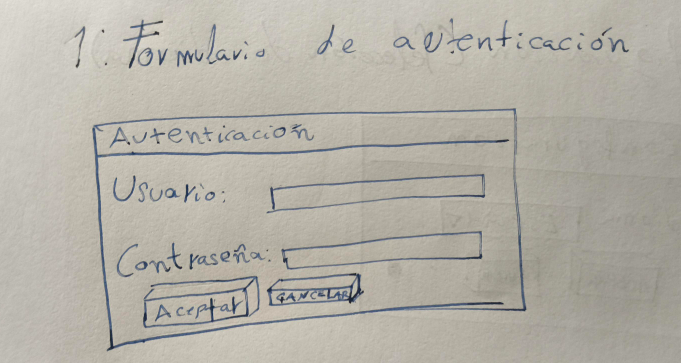
\includegraphics[width=300px,height=200px]{recursos/prototipos/autenticacion}
    \caption{Pantalla 1: Formulario de autenticación}
    \label{fig:autenticacion}
\end{figure}

\begin{figure}
    \centering
    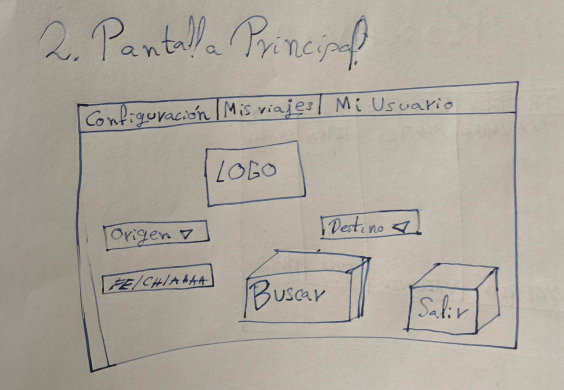
\includegraphics[width=300px,height=200px]{recursos/prototipos/pantalla_principal}
    \caption{Pantalla 2: Pantalla principal}
    \label{fig:pantalla_principal}
\end{figure}

\begin{figure}
    \centering
    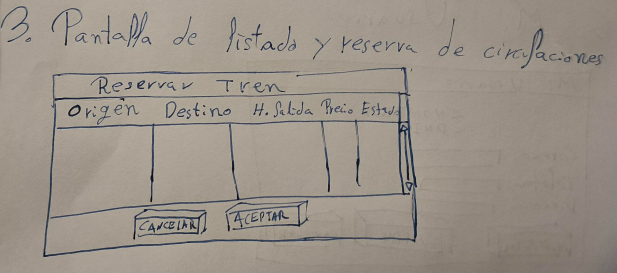
\includegraphics{recursos/prototipos/reservar_tren}
    \caption[width=120px,height=200px]{Pantalla 3: Lista de trenes y reserva de billetes}
    \label{fig:reservar_tren}
\end{figure}
\begin{figure}
    \centering
    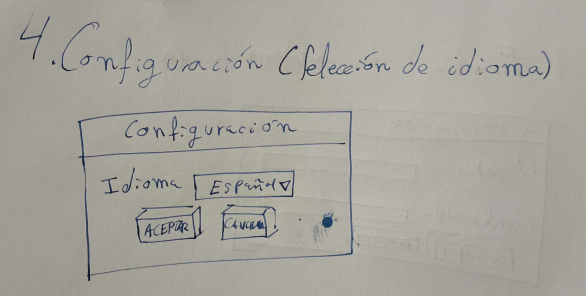
\includegraphics[width=300px,height=200px]{recursos/prototipos/elegir_idioma}
    \caption{Pantalla 4: Configuración}
    \label{fig:elegir_idioma}
\end{figure}

\begin{figure}
    \centering
    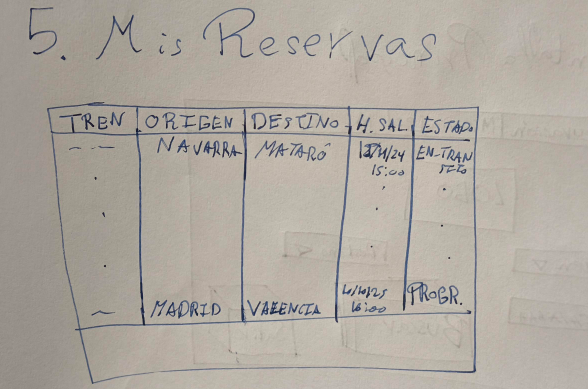
\includegraphics[width=300px,height=200px]{recursos/prototipos/mis_reservas}
    \caption{Pantalla 5: Mis Reservas}
    \label{fig:mis_reservas}
\end{figure}

\begin{figure}
    \centering
    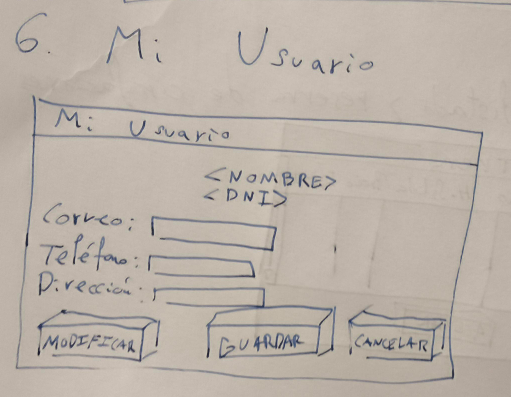
\includegraphics[width=300px,height=200px]{recursos/prototipos/mi_usuario}
    \caption{Pantalla 6: Mi usuario}
    \label{fig:mi_usuario}
\end{figure}


\newpage


\section{Diagramas UML}\label{sec:diagrama_de_clases}

\subsection{Diagrama de clases}\label{subsec:diagrama_de_clases}

Para comenzar, en la \autoref{fig:clases}, se muestran las clases que representan a la información que se maneja en la aplicación.

\begin{figure}[h]
    \centering
    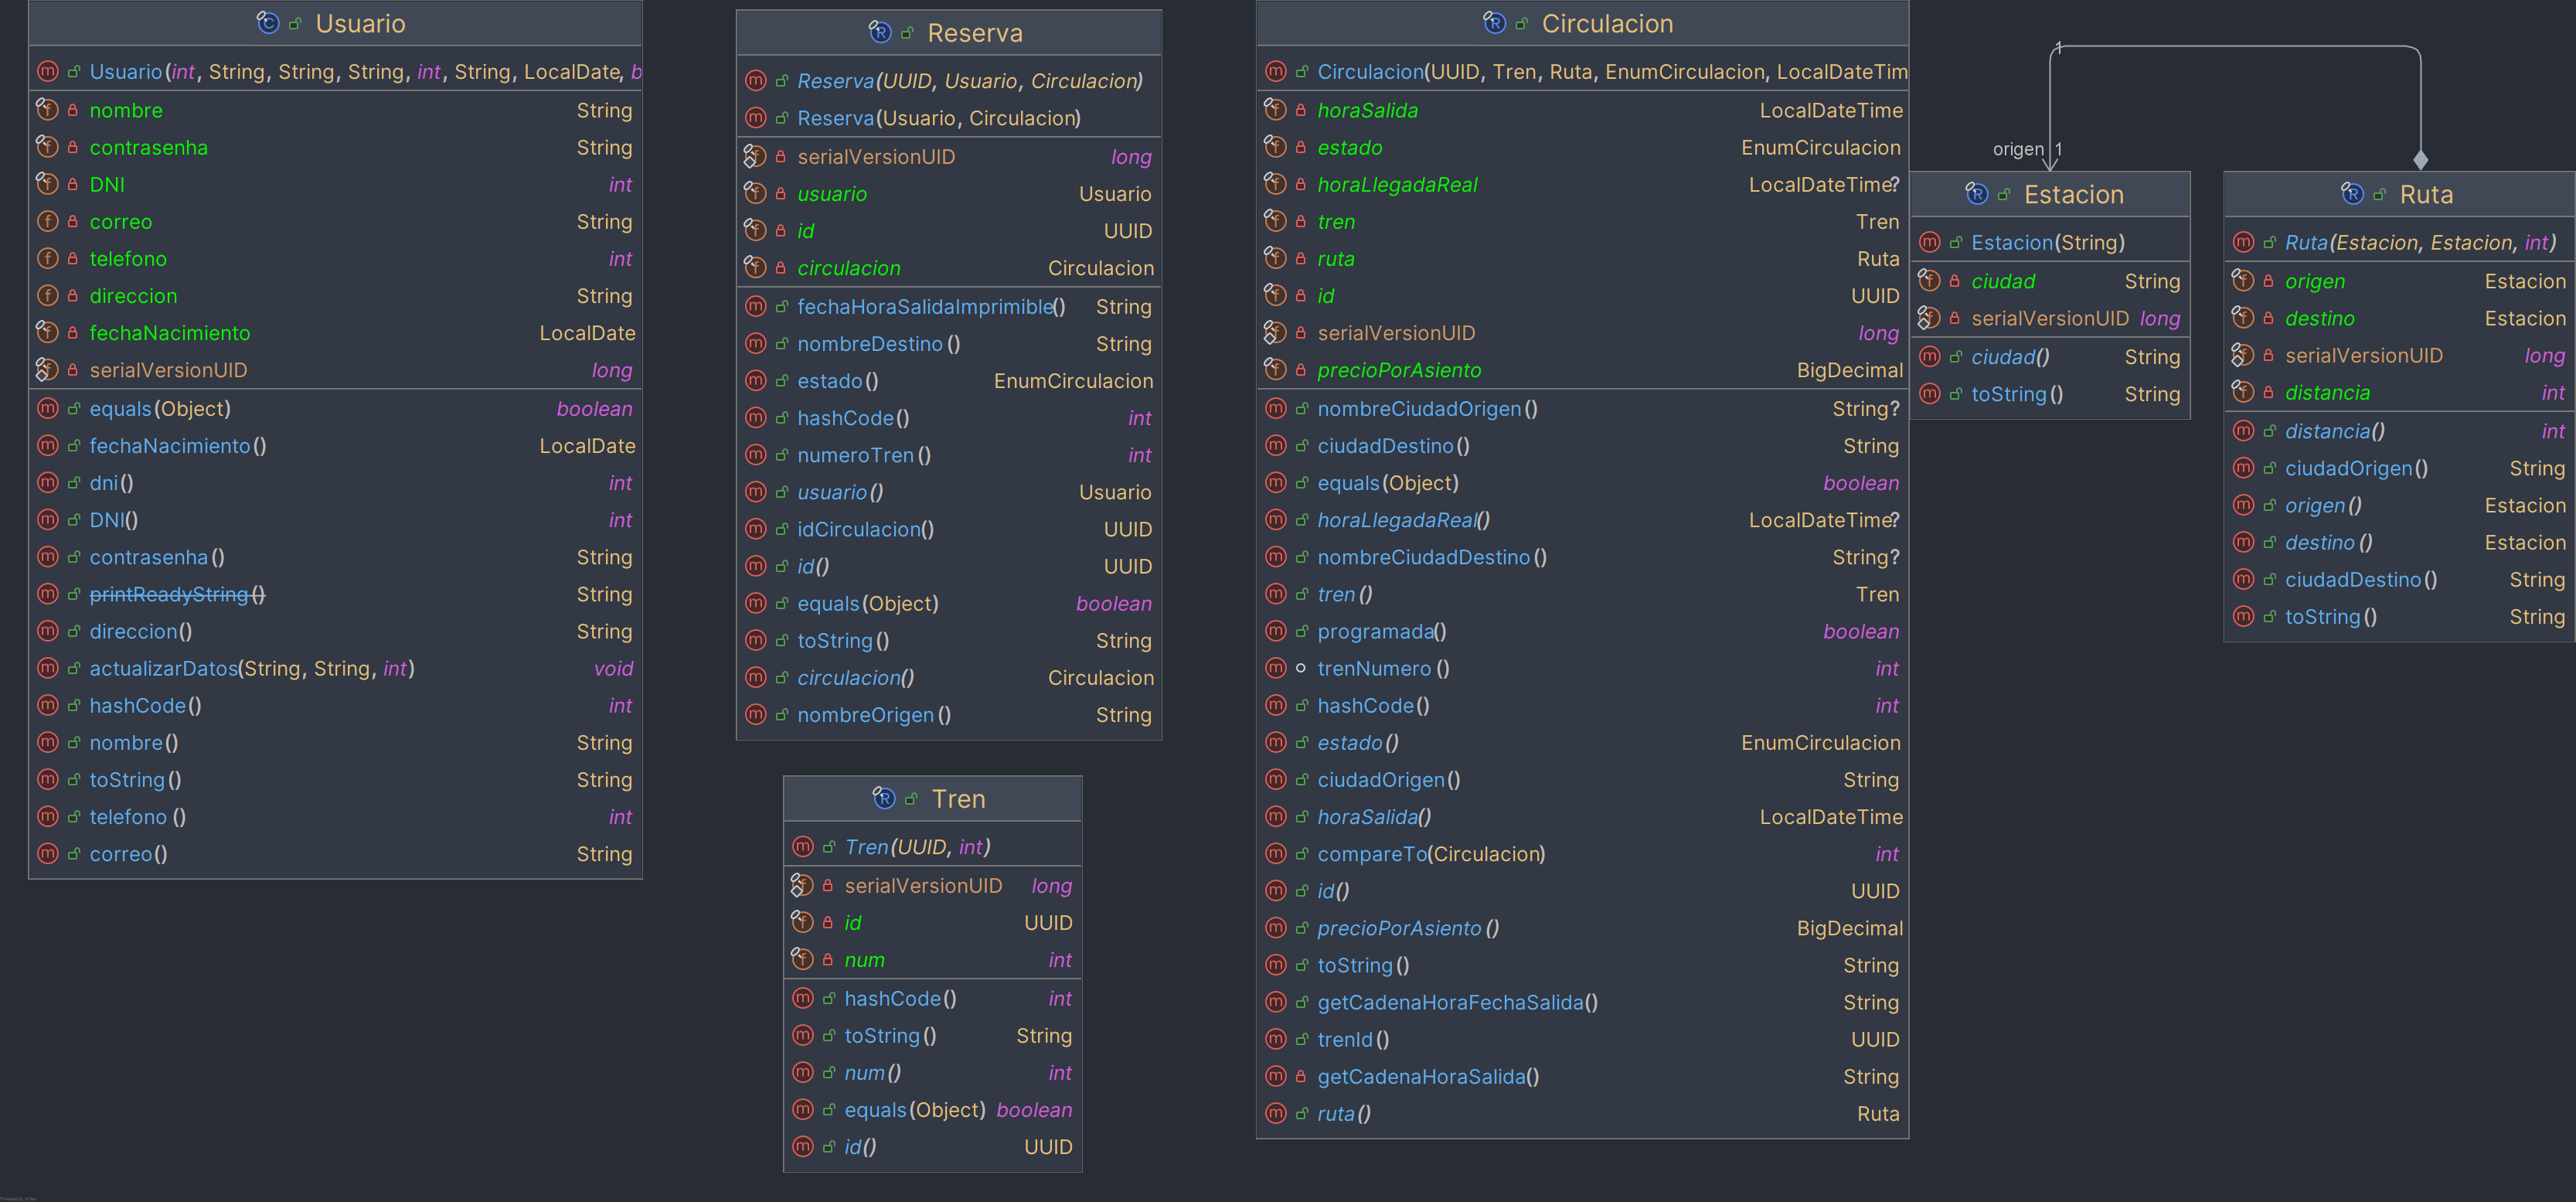
\includegraphics[width=260px]{recursos/diagramas/clases}
    \caption{Modelo de datos}
    \label{fig:clases}
\end{figure}

\subsection{Diagrama de clases DAO}\label{subsec:diagrama_de_clases_dao}

Relacionado con el modelo de datos, para implementar una persistencia o «serialización» de los datos, se ha implementado un patrón DAO (\textit{Data Access Object}).
El patrón DAO se encarga de abstraer la lógica de acceso a los datos (ver \autoref{sec:estructura}).
En la \autoref{fig:clases_dao} se muestra el diagrama de clases de este patrón.

En la implementación de este patrón, se han usado varias funcionalidades clave de Java.
Por un lado, la clase \textit{AbstractDAO} es una clase abstracta que implementa la interfaz \textit{IDAO}.
La clase AbstractDAO a su vez tiene una relación de herencia con los DAOs individuales.
\begin{figure}
    \centering
    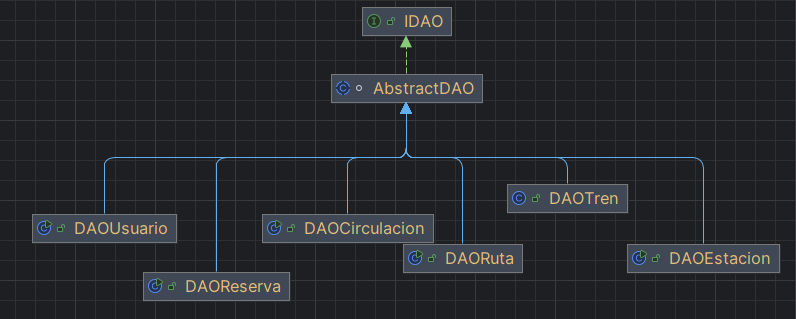
\includegraphics[width=200px]{recursos/diagramas/daoEstructura}
    \caption{Diseño de la estructura de clases del DAO}
    \label{fig:clases_dao}
\end{figure}

\subsection{Diagrama de clases GUI}\label{subsec:diagrama_de_clases_gui}
Llegados a este punto, se ha implementado la interfaz gráfica de usuario (GUI).
Se ha usado una estructura formulario-modelo para las clases GUI con tablas y elementos con información.
En la \autoref{fig:clases_gui} se muestra el diagrama de clases de la GUI\@.
\begin{figure}
    \centering
    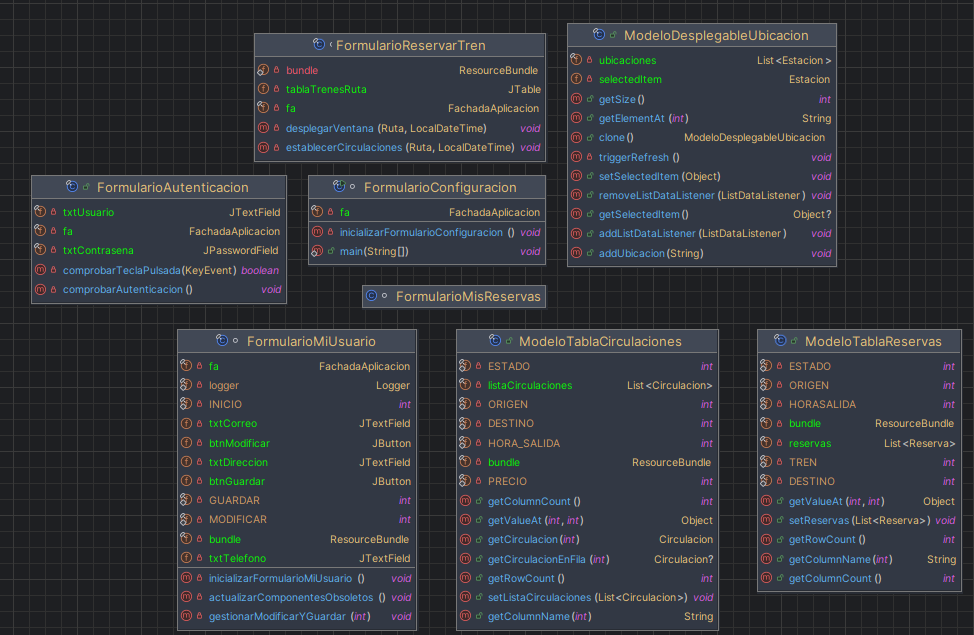
\includegraphics[width=200px]{recursos/diagramas/gui}
    \caption{Diagrama de clases para la interfaz gráfica}
    \label{fig:clases_gui}
\end{figure}

\subsection{Façade}\label{subsec:facade}
Para simplificar la interacción entre la GUI y el modelo de datos, se ha implementado un patrón Façade.
No solo simplifica la interacción, sino que también permite una mayor flexibilidad en la implementación de la GUI respecto al modelo de datos.
En la \autoref{fig:jerarquia_fachada} se muestra el diagrama de clases del Façade respecto a su jerarquía interna.

\begin{figure}
    \centering
    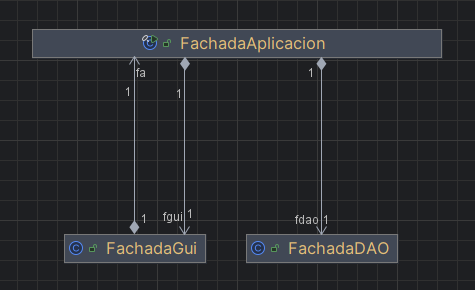
\includegraphics[width=200px]{recursos/diagramas/jerarquia_fachada}
    \caption{Jerarquia de clases para el patrón façade}
    \label{fig:jerarquia_fachada}
\end{figure}

Para poner un ejemplo, se puede ver como interactúan los DAOs con el Façade en la \autoref{fig:interaccion_fachada_dao}.

\begin{figure}
    \centering
    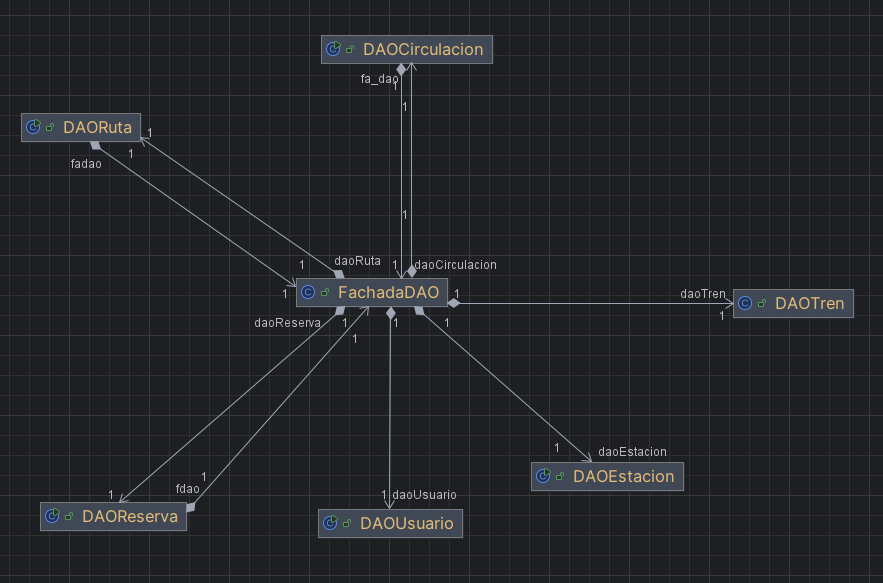
\includegraphics[width=200px]{recursos/diagramas/fdao_dao_rel}
    \caption{Relaciones entre la façada de los DAOs y los mismos DAOs}
    \label{fig:interaccion_fachada_dao}
\end{figure}

Estos son todos los diagramas UML más relevantes.
Se hablará más en detalle de la implementación en la \autoref{ch:implementacion}.
Respecto a la estructura del proyecto, se detalla a continuación en la \autoref{sec:estructura}.
\newpage


\section{Estructura del proyecto}\label{sec:estructura}
Para este apartado, seguiremos una lógica de aproximación top-down.
Analizaremos primero la estructura general del proyecto, para luego ir descendiendo en detalle. \footnote{Nota para el lector: Algunos patrones están repartidos entre este capítulo y el siguiente.}


 De esta forma iremos viendo cómo se ha estructurado el proyecto, desde la raíz hasta las clases más concretas.
A continuación, se muestra la estructura de directorios del proyecto en la \autoref{fig:estructura}.


\begin{figure}[h]
    \centering
    \framebox[\textwidth]{%
        \begin{minipage}{0.9\textwidth}

            \dirtree{%
                .1 TrainGo.
                .2 datos.
                .2 src.
            }
        \end{minipage}
    }
    \caption{Estructura de directorios del proyecto}
    \label{fig:estructura}
\end{figure}

Dentro del directorio \textit{datos}, habremos de hallar los archivos de datos que se usan en la aplicación.
Estos están escritos en un formato XML\@.

En el directorio \textit{src}, se encuentran los archivos fuente del proyecto, donde se encuentra la implementación de la aplicación.

El código fuente de esta aplicación sigue una modificación \textbf{patrón Modelo-Vista-Controlador} (MVC).
En este caso, se ha modificado el patrón para que se ajuste a las necesidades de la aplicación.
La estructura de directorios de la aplicación se muestra en la \autoref{fig:estructura_src}.

\begin{figure}[h]
    \centering
    \framebox[\textwidth]{%
        \begin{minipage}{0.9\textwidth}
            \dirtree{%
                .1 src.
                .2 main.
                .3 java.
                .4 com.
                .5 marceSoft.
                .6 trainGo.
                .7 aplicacion.
                .7 dao.
                .7 gui.
                .7 util.
                .3 resources.
                .4 images.
            }
        \end{minipage}
    }
    \caption{Estructura de directorios del código fuente}
    \label{fig:estructura_src}
\end{figure}

En el directorio \textit{aplicacion}, se encuentran las clases que implementan la lógica de la aplicación
y los modelos de datos.
(es decir, modelo y controlador).

En el directorio \textit{dao}, se encuentran las clases que implementan el patrón DAO\@.
Es importante separar la lógica de acceso a los datos de la lógica de la aplicación,
ya que al hacerlo, se facilita la implementación de la persistencia de los datos.

En el directorio \textit{gui}, se encuentran las clases que implementan la interfaz gráfica de usuario.
Estas clases se encargan de mostrar la información al usuario y de recibir la información del usuario (vista).

En el directorio \textit{util}, se encuentran las clases que implementan utilidades para la aplicación.

En el directorio \textit{resources}, hallamos los \textit{bundles} de internacionalización,
archivo de configuración del \textit{logger} y las imágenes que se usan en la aplicación.
Sin embargo, es mejor no adelantarse, ya trataremos estos aspectos en el \autoref{ch:implementacion}.

\newpage

\subsection{Estructura del paquete \textit{aplicacion}}\label{subsec:estructura_del_paquete_aplicacion}
Volviendo a la estructura de paquetes, en el paquete \textit{aplicacion} se encuentran las clases que implementan parte de la lógica de la aplicación.

Por un lado, tenemos la \textit{FachadaAplicacion}, que se encarga de abstraer la lógica de la aplicación. \footnote{ En la \autoref{fig:jerarquia_fachada} se muestra la jerarquía de clases de la Fachada.}
Al mismo nivel, se encuentran las clases «contenedoras» de los modelos de datos.

Bajando un nivel nos podemos encontrar con la anotación \textit{NoNegativo} y su validador,
los dos enums, las excepciones y formateadores personalizados.
Esto se ve muy bien en la \autoref{fig:estructura_aplicacion}.

\begin{figure}[h]
    \centering
    \framebox[\textwidth]{%
        \begin{minipage}{0.9\textwidth}
            \dirtree{%
                .1 aplicacion.
                .2 anotaciones.
                .3 validadores.
                .4 ValidadorNoNegativo.java.
                .3 NoNegativo.java.
                .2 enums.
                .3 EnumCirculacion.java.
                .3 EnumIdioma.java.
                .2 excepciones.
                .3 CargaArchivoFallidaException.java.
                .3 CierreArchivoXMLErroneoException.java.
                .3 LecturaSiguienteEventoException.java.
                .3 NoHayUsuariosRegistradosException.java.
                .3 ProcesadoSiguieteEventoException.java.
                .3 SituacionDeRutasInesperadaException.java.
                .3 UsuarioNoEncontradoException.java.
                .2 formato.
                .3 FormattedFecha.java.
                .2 FachadaAplicacion.java.
                .2 Circulacion.java.
                .2 Estacion.java.
                .2 Reserva.java.
                .2 Ruta.java.
                .2 Tren.java.
                .2 Usuario.java.
            }
        \end{minipage}
    }
    \caption{Estructura de clases del paquete \textit{aplicacion}}
    \label{fig:estructura_aplicacion}
\end{figure}

De esta zona, lo más reseñable a nivel de diseño, es, tal vez, es la decisión de poner Usuario
como clase contenedora modificable, mientras que el resto de clases son inmutables (\textit{Records}).
Esto se debe a que los usuarios son los únicos datos que son susceptibles a cambios.

Otra vez, se me puede (con cierta razón) acusar de adelantarme.
Permitidme, entonces, que me disculpe y que os remita al \autoref{ch:implementacion} para más detalles.
Sin embargo, considero que es una decisión de diseño importante,
ya que aunque hay datos que pueden ser «renovados» (como las reservas),
una reserva «modificada» es, en realidad, una reserva nueva (en nuestro caso).
Por este motivo, se ha decidido que las reservas sean inmutables.

\subsection{Estructura del paquete \textit{dao}}\label{subsec:estructura_del_paquete_dao}
En el paquete \textit{dao}, se encuentran las clases que implementan el patrón DAO,
que se encarga de abstraer la lógica de acceso a los datos (persistencia).

Este paquete está estructurado como se muestra en la \autoref{fig:estructura_dao}.

\begin{figure}[h]
    \centering
    \framebox[\textwidth]{%
        \begin{minipage}{0.9\textwidth}
            \dirtree{%
                .1 dao.
                .2 constantes.
                .2 FachadaDAO.java.
                .2 IDAO.java.
                .2 AbstractDAO.java.
                .2 DAOCirculacion.java.
                .2 DAOEstacion.java.
                .2 DAOReserva.java.
                .2 DAORuta.java.
                .2 DAOTren.java.
                .2 DAOUsuario.java.
            }
        \end{minipage}
    }
    \caption{Estructura de clases del paquete \textit{dao}}
    \label{fig:estructura_dao}
\end{figure}


En este paquete, se ha implementado un patrón DAO para abstraer la lógica de acceso a los datos.
Este ha sido implementado siguiendo una versión simplificada de las directrices oficiales de ORACLE~\autocite
{oracle.dao},
que también es usado por otros autores~\autocite{baeldung.dao}.

La toma de decisiones en este paquete ha sido más sencilla,
ya que se ha seguido una estructura de clases más estándar.

Siguiendo el patrón previamente mencionado, se ha implementado una interfaz \textit{IDAO} que define los métodos que deben implementar los DAOs.
En este caso, se ha añadido una clase abstracta \textit{AbstractDAO} que implementa la interfaz \textit{IDAO}.
Todo esto se puede ver en la \autoref{fig:clases_dao}.

Hay un paquete más dentro del paquete \textit{dao}, que puede pasar fácilmente desapercibido.
Este paquete es el de las constantes.
Su distribución se muestra en la \autoref{fig:estructura_dao_constantes}.

\begin{figure}[h]
    \centering
    \framebox[\textwidth]{%
        \begin{minipage}{0.9\textwidth}
            \dirtree{%
                .1 dao.
                .2 constantes.
                .3 ConstantesGeneral.java.
                .3 TagsXMLCirculacion.java.
                .3 TagsXMLEstacion.java.
                .3 TagsXMLReserva.java.
                .3 TagsXMLRuta.java.
                .3 TagsXMLTren.java.
                .3 TagsXMLUsuario.java.
            }
        \end{minipage}
    }
    \caption{Estructura de clases del paquete \textit{dao}}
    \label{fig:estructura_dao_constantes}
\end{figure}

En este paquete, se encuentran las constantes que se usan en los DAOs.

\subsection{Estructura del paquete \textit{gui}}\label{subsec:estructura_del_paquete_gui}
Saliendo de la espesura de los DAOs, nos encontramos con el paquete \textit{gui}.

Este paquete contiene las clases que implementan la interfaz gráfica de usuario.
La estructura de este paquete se muestra en la \autoref{fig:estructura_gui}.
\begin{figure}[h]
    \centering
    \framebox[\textwidth]
    {%
        \begin{minipage}{0.9\textwidth}
            \dirtree{%
                .1 gui.
                .2 FachadaGUI.java.
                .2 formularios.
                .2 modelos.
            }
        \end{minipage}
    }
    \caption{Estructura de clases del paquete \textit{gui}}
    \label{fig:estructura_gui}
\end{figure}

Es un paquete relativamente sencillo con una estructura bastante intuitiva.
Por un lado, tenemos la habitual façada, que se encarga de abstraer la lógica de la interfaz gráfica.
Y, nos quedan los formularios y los modelos.

Si desviamos la mirada hacia los formularios, nos encontramos con todos los formularios que se usan en la aplicación.
La estructura de este paquete se muestra en la \autoref{fig:estructura_gui_formularios}.

\begin{figure}[h]
    \centering
    \framebox[\textwidth]
    {%
        \begin{minipage}{0.9\textwidth}
            \dirtree{%
                .1 gui.
                .2 formularios.
                .3 FormularioAutenticacion.java.
                .3 FormularioConfiguracion.java.
                .3 FormularioMisReservas.java.
                .3 FormularioMiUsuario.java.
                .3 FormularioPrincipal.java.
                .3 FormularioReservarTren.java.
            }
        \end{minipage}
    }
    \caption{Estructura de clases del paquete \textit{gui}}
    \label{fig:estructura_gui_formularios}
\end{figure}

Pero, ¿qué es ese paquete \textit{modelos} que se ve en la \autoref{fig:estructura_gui}?
Pues, es un paquete que contiene los modelos de las tablas que se usan en la aplicación.

La estructura de este paquete se muestra en la \autoref{fig:estructura_gui_modelos}.

\begin{figure}[h]
    \centering
    \framebox[\textwidth]
    {%
        \begin{minipage}{0.9\textwidth}
            \dirtree{%
                .1 gui.
                .2 modelos.
                .3 ModeloDesplegableUbicacion.
                .3 ModeloTablaCirculaciones.
                .3 ModeloTablaReservas.
            }
        \end{minipage}
    }
    \caption{Estructura de clases del paquete \textit{gui}}
    \label{fig:estructura_gui_modelos}
\end{figure}

En este paquete, se encuentran los modelos de las tablas que se usan en la aplicación.

\subsection{Estructura del paquete \textit{util}}\label{subsec:estructura_del_paquete_util}
Por último, nos encontramos con el paquete \textit{util}.
Este paquete es trivial, ya que solo contiene clases de utilidades.
Contamos tres clases en este paquete: \textit{Criptograficos}, \textit{Internacionalizacion} y \textit{Ortograficos}.

Para no hacer un «look-ahead», ya hablamos ahora de sus propósitos en el capítulo de la implementación de la aplicación.

\newpage

\section{Herramientas, tecnologías y librerías}\label{sec:herramientas_tecnologias_y_librerias}
Para la implementación de la aplicación, se han usado varias herramientas, tecnologías y librerías.
A continuación, se detallan las más relevantes (obviaré las más obvias, como Java 22).

Para generar los diagramas UML, JavaDocs y como IDE de desarrollo, se ha usado IntelliJ IDEA~\autocite{jetbrains.idea}.

Para la gestión de dependencias, se ha usado Maven~\autocite{maven}.
Maven es una herramienta de gestión de proyectos que se encarga de la gestión desde las dependencias hasta la compilación (y más allá).

Para la generación de datos «dummy», se ha utilizado la página web \textit{Mockaroo}~\autocite{mockaroo}.
Mockaroo es una herramienta que permite generar datos de prueba de forma aleatoria.

Para la creación de este informe, se ha usado \LaTeX{}.

Pasando a las librerías, se han usado las siguientes:
\begin{itemize}
    \item logback~\autocite{logback} para el registro de eventos (logging).
    \item Jetbrains Annotations~\autocite{jetbrains.annotations} para las anotaciones.
\end{itemize}

Finalmente, se ha hecho uso del estándar XML (eXtensible Markup Language) para el almacenamiento de los datos.

\newpage
